% Drawing 156-8/05-3 -- folder 156-8, batch 05, archive page 97 (PDF page 98).
% Transcription: deux segments contigus, de sommets $a$, $b$, $c$.
% Kind: two contiguous segments. Method 3 (encoded, rendered from the data). Status: ok.
% Notes: Two contiguous segments [a, b], [b, c].
% Coordinates: 1 unit = 1 mm = 1/100 of the crop width (bbox in page fractions: [0.28, 0.48, 0.62, 0.56]).
% Redrawn by Claude (claude-opus-5-5), issue #73 pilot, 2026-11-07; not checked by a human; not compiled (no TeX in the session).
% Rights: reproduces part of the work -- behind RENDER_TRANSCRIPTS, never published by itself.
\documentclass[tikz,border=3pt]{standalone}
\usepackage{amsmath,amssymb}
\usetikzlibrary{patterns,arrows.meta}
\tikzset{pencil/.style={black!45}, struck/.style={black!35}, mark/.style={circle,draw,inner sep=1.3pt}, pt/.style={circle,fill,inner sep=0.9pt}, opt/.style={circle,draw,fill=white,inner sep=1.1pt}}
\begin{document}
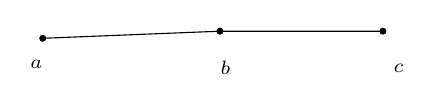
\begin{tikzpicture}[x=1mm,y=1mm,line cap=round,line join=round,font=\scriptsize]
\draw (25.8,-24.7) -- (48.3,-23.8) -- (69,-23.8);
\node[pt] at (25.8,-24.7) {};
\node[pt] at (48.3,-23.8) {};
\node[pt] at (69,-23.8) {};
\node[inner sep=1pt] at (25,-28) {\scriptsize $a$};
\node[inner sep=1pt] at (49,-28.5) {\scriptsize $b$};
\node[inner sep=1pt] at (71,-28.5) {\scriptsize $c$};
\end{tikzpicture}
\end{document}
